%%%%%%%%%%%%%%%%%%%%%%%%%%%%%%%%%%%%%%%%%
% Simple Sectioned Essay Template
% LaTeX Template
%
% This template has been downloaded from:
% http://www.latextemplates.com
%
% Note:
% The \lipsum[#] commands throughout this template generate dummy text
% to fill the template out. These commands should all be removed when 
% writing essay content.
%
%%%%%%%%%%%%%%%%%%%%%%%%%%%%%%%%%%%%%%%%%

%----------------------------------------------------------------------------------------
%	PACKAGES AND OTHER DOCUMENT CONFIGURATIONS
%----------------------------------------------------------------------------------------

\documentclass[12pt]{article}

\usepackage[italian]{babel}
\usepackage[utf8]{inputenc}
\usepackage{geometry}
\usepackage{graphicx}
\usepackage{float}
\usepackage{wrapfig}
\usepackage[dvipsnames]{xcolor}
\usepackage{acronym}
\usepackage{lipsum}
\usepackage{listings}
\usepackage{mathtools}
\usepackage{hyperref}
\usepackage[object=vectorian]{pgfornament}
\usepackage{tikz}

\geometry{a4paper}

\linespread{1.1}

\graphicspath{{img/}}

\definecolor{back}{rgb}{1,0.93,0.76} 
\lstset{ %
	backgroundcolor=\color{back},  	% choose the background color; you must add \usepackage{color} or \usepackage{xcolor}; should come as last argument
	basicstyle=\tiny,        		% the size of the fonts that are used for the code
	breakatwhitespace=false,        % sets if automatic breaks should only happen at whitespace
	breaklines=true,                % sets automatic line breaking
	captionpos=b,                   % sets the caption-position to bottom
	commentstyle=\color{gray},   	% comment style
	frame=single,	                % adds a frame around the code
	frameround=tttt					% round corner (use f instead t to edge corner)
	keepspaces=true,                % keeps spaces in text, useful for keeping indentation of code (possibly needs columns=flexible)
	keywordstyle=\color{blue},      % keyword style
	language=Python,               	% the language of the code
	numbers=none,                   % where to put the line-numbers; possible values are (none, left, right)
	numbersep=5pt,                  % how far the line-numbers are from the code
	numberstyle=\tiny\color{black}, % the style that is used for the line-numbers
	rulecolor=\color{black},        % if not set, the frame-color may be changed on line-breaks within not-black text (e.g. comments (green here))
	showspaces=false,               % show spaces everywhere adding particular underscores; it overrides 'showstringspaces'
	showstringspaces=false,         % underline spaces within strings only
	showtabs=false,                 % show tabs within strings adding particular underscores
	stepnumber=1,                   % the step between two line-numbers. If it's 1, each line will be numbered
	stringstyle=\color{OrangeRed},  % string literal style
	tabsize=2                   	% sets default tabsize to 2 spaces
}

\acrodef{PCA}{\emph{Principal Component Analysis}}

\newcommand{\codice}[2]{\lstinputlisting[firstline=#1, lastline=#2]{code/PCA.py}}

\newcommand{\sectionline}{
	\begin{center}
		\resizebox{0.5\linewidth}{1ex}{
			\begin{tikzpicture}
			\node  (C) at (0,0) {};
			\node (D) at (9,0) {};
			\path (C) to [ornament=83] (D);
			\end{tikzpicture}
		}
	\end{center}
}

\begin{document}

%----------------------------------------------------------------------------------------
%	TITLE PAGE
%----------------------------------------------------------------------------------------

\begin{titlepage}

\newcommand{\HRule}{\rule{\linewidth}{0.5mm}}

\center

\textsc{\LARGE Università degli studi di Firenze}\\[1.5cm]
\textsc{\Large Corso di Laurea Magistrale in Informatica}\\[0.5cm]
\textsc{\large Advanced Techniques and tools for software development}\\[0.5cm]

\HRule \\[0.4cm]
{ \huge \bfseries Integrazione parte web}\\[0.4cm]
\HRule \\[1.5cm]

\begin{minipage}{0.4\textwidth}
	\begin{flushleft} \large
		\emph{Autore:}\\
		Marco \textsc{Buracchi}
	\end{flushleft}
\end{minipage}
~
\begin{minipage}{0.4\textwidth}
	\begin{flushright} \large
		\emph{Docente:} \\
		Prof Lorenzo \textsc{Bettini}
	\end{flushright}
\end{minipage}\\[4cm]

{\large \today}\\[3cm] % Date, change the \today to a set date if you want to be precise
\vfill % Fill the rest of the page with whitespace

\end{titlepage}

%----------------------------------------------------------------------------------------
%	TESTO
%----------------------------------------------------------------------------------------

\section{Cenni preliminari}

	In questo progetto è stata creata una applicazione web utilizzando il framework \emph{Spring}. Questa applicazione permette di cifrare e decifrare stringhe di testo utilizzando due cifrari:
	
	\begin{itemize}
		\item Shift cipher
		\item Vigenere cipher
	\end{itemize}
	
	Per utilizzare questi due cifrari che fanno parte del progetto precedentemente sviluppato si è ricorso all'utilizzo dei moduli di \emph{MAVEN}. \'{E} stato infatti creato un parent POM che gestisse le dipendenze necessarie all'interazione tra i due moduli interessati.
	
	\subsection{Struttura progetto}
		Le quattro classi principali che implementano l'applicazione sono \emph{Cifrario, CipherService, CiphersWebController} e \emph{TapWebIntegrationApplication}.
		
		Per quanto riguarda i test, sono presenti tre classi di unit-testing (non è stato testata la classe \emph{Cifrario} che funge da modello) e tre classi di integration-testing per controllare l'effettivo funzionamento dell'interazione tra le varie componenti dell'applicazione e un test \emph{end to end}.
		
		Sono presenti anche 6 pagine \emph{html} e due file \emph{css}.
	
	\sectionline
	
\section{Strumenti utilizzati}
	\begin{description}
		\item[Maven:] Maven è stato utilizzato per gestire le varie dipendenze del progetto e la build automatica. \`{E} stato quindi creato un progetto Maven separato che funga da progetto \emph{parent} che collega il modulo core al modulo web.
		
		\item[GitHub:] La repository contenente il progetto è raggiungibile tramite questo link \url{https://github.com/ma-buracchi/TAP-Integrazione}.
		
		\item[Travis:] Travis viene utilizzato per la continuous integration. Il relativo file di configurazione è stato settato per utilizzare la jdk8 necessaria alla compilazione del progetto e per fornire il risultato dell'analisi a \emph{SonarCloud}. Il risultato della scansione è visibile in figura \ref{fig:sonar}.
		
		\begin{figure}
			\begin{center}
				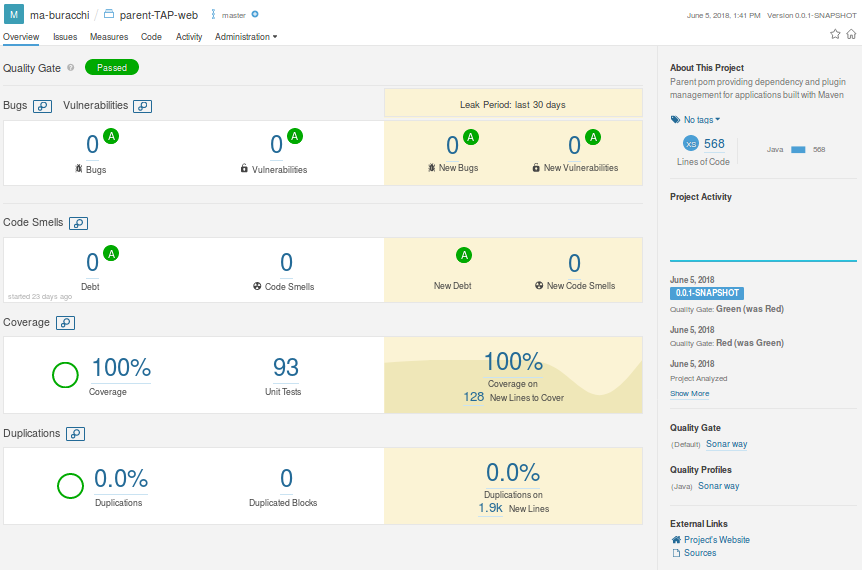
\includegraphics[scale=.3]{img/sonarCloud}
				\caption{Analisi sonarCloud}
				\label{fig:sonar}
			\end{center}
		\end{figure}
		
		Una build automatica viene lanciata ad ogni push effettuata sul repository GitHub contenente il progetto.
		
		Il progetto è raggiungibile al seguente link: \url{https://travis-ci.org/ma-buracchi/TAP-Integrazione}.
		
		\item[Spring Framework:] Il framework Spring è stato utilizzato per la creazione e il testing dell'app. Essa è infatti una SpringBoot Application che viene lanciata in locale su \url{http://localhost:8080} direttamente da Eclipse tramite la SpringTool Suite. Lo stesso framework viene utilizzato anche per il testing.
		
		\item[HTMLUnit:] Questo framework è stato utilizzato in questo progetto per effettuare degli end to end testing.
	\end{description}
	
\section{Testing}
	Come detto, la classe \emph{Cifrario} non è stata testata in quanto contiene solamente metodi getters e setters.
	
	La classe \emph{CipherService} è stata testata verificando il comportamento dei due cifrari utilizzabili. Utilizzando i Mock di \emph{Cifrario}, \emph{Vigenere} e \emph{Shift} è stato possibile testare la classe in isolamento. I comportamenti testati sono la cifratura/decifratura con entrambi i cifrari. Non è stato ritenuto necessario testare il comportamento della classe con dati mancanti in quanto devono essere forniti obbligatoriamente dall'utente.
	
	Per quanto riguarda il \emph{CiphersWebController} sono stati testati i pulsanti della barra di navigazione (Home e About), lo status 200 della homepage, la selezione dei due cifrari e la corretta visualizzazione dei loro risultati.
	
	Sono poi stati effettuati degli Integration Testing per verificare la corretta interazione tra il Service e un istanza di Vigenere, tra il Service e un'istanza di Shift e tra il Controller, il Service e il Cifrario.
	
	Per ultimo è stato effettuato un test \emph{end to end} utilizzando HTMLUnit.

\end{document}